\chapter*{Załącznik A: Instrukcja użycia biblioteki}
\addcontentsline{toc}{chapter}{Załącznik A: Instrukcja użycia biblioteki}
\markboth{}{Załącznik A: Instrukcja użycia biblioteki}
W załączniku opisana została procedura użycia modułu URM w formie poradnika utworzenia przykładowego projektu i skonfigurowania go pod potrzeby biblioteki. Do przykładu użyty zostanie program Visual Studio 2022 z zainstalowanym pakietem \textbf{Game development with C++} oraz zintegrowany z nim system budowy MSBuild. Do instalacji pakietów posłuży skonfigurowany do pracy z Visual Studio program \textbf{vcpkg} od firmy Microsoft. 

Biblioteka może zostać zaimportowana w dwóch trybach:
\begin{enumerate}
	\item \textbf{Prekompilowana} - forma dystrybucji, w której moduł przyjmuje formę gotowych do użycia plików .lib, zawierających skompilowane funkcje biblioteki. Dzięki takiemu podejściu można uniknąć każdorazowego rekompilowania kodu przy tworzeniu projektu, a także potencjalnych problemów z kompatybilnością między różnymi wersjami kompilatora. 
	\item \textbf{Kod źródłowy} - bezpośrednie dodanie projektów wraz z kodem źródłowym jako referencji do aplikacji klienta. W takim przypadku możliwa jest dowolna modyfikacja kodu biblioteki, ale kosztem konieczności jej ręcznego skompilowania oraz trudniejszej aktualizacji.
\end{enumerate}

\section*{Wspólna konfiguracja projektu}
Niezależnie od wybranej wersji wymaganym od projektu jest ustawienie kilku kluczowych opcji konfiguracyjnych oraz przygotowań.

Wewnątrz kodu źródłowego biblioteki dostępnego na stronie projektu \cite{GitHub:Minik:MasterThesisUniversalRenderingModuleD3D11} znajdują się skrypty automatyzujące instalację wymaganych do działania bibliotek. Są to \textbf{vcpkg\_install.bat} oraz \textbf{vcpkg\_install\_x86.bat}, odpowiednio dla wersji 64bit i 32bit. Skrypty wywołują program \textit{vcpkg} z odpowiednimi parametrami, dzięki czemu można uniknąć ręcznej instalacji wymaganych bibliotek. Tej operacji nie trzeba powtarzać dla kolejnych projektów, gdyż vcpkg przechowuje zainstalowane biblioteki we współdzielonej lokalizacji. Alternatywą bez konieczności instalacji vcpkg jest ręczne zainstalowanie bibliotek \textbf{directxtk}, \textbf{spdlog} oraz \textbf{assimp}.

Ze względu na wykorzystanie zaawansowanych konceptów jak \textit{std::variant} i \textit{concepts}, moduł do swojego działania wymaga języka w wersji \textbf{C++20} lub nowszej. Dodatkowo do poprawnej kompilacji wymagana jest także flaga \textbf{/utf-8}, która wymusza na kompilatorze użycie kodowania UTF-8. Na koniec do poprawnego działania z WinAPI koniecznym jest też przestawienie użytego subsystemu na \textbf{Windows}.

Warto jest też ustawić parametr \textit{Debugging -> Working Directory} na wartość \textbf{\$(OutputPath)}, gdyż umożliwi to wczytywanie zasobów z katalogu wynikowego, do którego będą one automatycznie trafiać przy kompilacji.

Poniżej znajduje się podsumowanie wymaganych ustawień:

\begin{center}
	\begin{tabular}{ |l r|}
		\hline
		\textbf{Ustawienie} & \textbf{Wartość} \\
		\hline
		General -> \textbf{C++ language standard}  & \textbf{>= C++20} \\
		C/C++ -> Command Line -> \textbf{Additional Options} & \textbf{/utf-8} \\
		Linker -> System -> \textbf{SubSystem} & \textbf{Windows} \\
		*Debugging -> Working Directory & \textbf{\$(OutputPath)} \\
		\hline
	\end{tabular}
\end{center}

\section*{Tryb prekompilowany}
Pierwszym krokiem jest pobranie najnowszego pliku URM.zip z zakładki Releases ze strony projektu \cite{GitHub:Minik:MasterThesisUniversalRenderingModuleD3D11}. Zawiera on 3 katalogi:

\begin{itemize}
	\item \textbf{bin} - pliki konieczne do działania gotowego programu.
	\item \textbf{include} - pliki nagłówkowe używane jako referencja do kodu źródłowego.
	\item \textbf{lib} - prekompilowane pliki modułu używane do kompilacji. 
\end{itemize}

Wspomniane katalogi należy rozpakować do wybranego folderu, najlepiej znajdującego się w ramach katalogu aplikacji klienckiej. W następnym kroku należy we właściwościach projektu wskazać lokalizację komponentów według następującego schematu:

\begin{itemize}
	\item \textbf{C/C++ -> General -> Additional Include Directories}: ścieżka do katalogu \textbf{include} wewnątrz wypakowanego folderu. 
	\item \textbf{Linker -> General}: ścieżka do katalogu \textbf{lib} według następującego schematu: \textbf{(...)/lib/\{MODE\}/\{ARCH\}}, gdzie jako \textbf{\{MODE\}} należy ustawić wybrany tryb kompilacji \textbf{(Release / Debug)}, a jako \textbf{\{ARCH\}} wybraną architekturę \textbf{(x86/x64)}. Przykład: \textit{(...)/lib/Release/x64} Operację powtórzyć należy dla każdej docelowej kombinacji tych dwóch wartości, zmieniając je na górnej części okna właściwości. 
	\item \textbf{Linker -> Input -> Additional Dependencies}: wykorzystywane biblioteki. W przypadku użycia jedynie warstwy rdzeniowej należy dodać \textbf{URMCore.lib}, a używając modułu silnika dodatkowo także \textbf{URMEngine.lib}.
\end{itemize}

Ostatnim ważnym krokiem jest dodanie plików z katalogu \textbf{bin} jako zasobów do projektu aplikacji. Następnie po zaznaczeniu nowo dodanych plików należy wejść w ich właściwości i w \textbf{General -> Item Type} skonfigurować jako \textbf{Copy File}. W ten sposób pliki zostaną przekopiowane do katalogu wynikowego przy kompilacji, gdzie będą dostępne do użycia przez moduły i aplikację. 

\section*{Tryb kodu źródłowego}
Podobnie jak w poprzedniej sekcji pierwszym krokiem jest pobranie najnowszej wersji biblioteki, ale w tym przypadku w formie kodu źródłowego. Można tego dokonać na 2 sposoby:
\begin{itemize}
	\item Pobierając \textbf{Source Code (zip)} z zakładki Releases ze strony projektu \cite{GitHub:Minik:MasterThesisUniversalRenderingModuleD3D11}, a następnie wypakowując do wybranego folderu, najlepiej wewnątrz katalogu aplikacji.
	\item Wykonując klon kodu przy pomocy narzędzia git i dodając go jako submoduł do plików projektu. Zalecane w przypadku chęci wykonania modyfikacji, gdyż po wykonaniu operacji \textit{Fork} możliwe jest zachowanie możliwości aktualizacji także po własnych zmianach.
\end{itemize}

Projekty bibliotek znajdować się będą w katalogu \textbf{(...)/lib/URM/}. Aby użyć ich z aplikacją klienta należy dodać projekty do rozwiązania przy pomocy Visual Studio, w którym po kliknięciu prawym przyciskiem myszki na otwarte rozwiązanie należy wybrać \textbf{Add -> Existing Project} i wskazać pliki \textit{.vcxproj} docelowych modułów. Używając biblioteki rdzeniowej należy dodać \textbf{(...)/lib/URM/Core/Core.vcxproj}, a jeśli założeniem jest także użycie modułu silnika należy powtórzyć operację dla \textbf{(...)/lib/URM/Engine/Engine.vcxproj}.

Następnym krokiem wewnątrz programu Visual Studio jest dodanie referencji do nowych bibliotek. Można tego dokonać klikając prawym przyciskiem myszy na projekt aplikacji, a następnie wybierając \textbf{Add -> Reference}. Z nowego okna wybrać należy moduły, których zamierza się użyć.

Ostatnim elementem koniecznym do działania jest wskazanie lokalizacji dla plików nagłówkowych. Jest to możliwe poprzez dodanie ścieżki do katalogu \textbf{(...)/lib} do pola \textbf{C/C++ -> General -> Additional Include Directories} we właściwościach projektu.

Pliki zasobów silnika zostaną automatycznie skompilowane i przeniesione do wynikowego folderu, także nie trzeba na tym polu nic dodatkowo konfigurować. 

\section*{Przykładowa aplikacja testowa}
Po dostosowaniu ustawień warto przetestować poprawność konfiguracji. Najlepiej dokonać tego przez próbę skompilowania i uruchomienia testowego programu, wykorzystującego nowo dodaną bibliotekę. Moduł Engine wykorzystuje wewnętrznie moduł rdzeniowy, także nie jest konieczne jego osobne sprawdzanie jeśli w planach jest użycie modułu wysokopoziomowego. 

\subsection*{Warstwa rdzeniowa}
Do przetestowania poprawności konfiguracji projektu korzystającego z warstwy rdzeniowej można użyć programu pokazanego na listingu \ref{lst:appendix:coreDemo}. Jest to proste demo, które w pętli czyści i wyświetla zawartość nowo otwartego okna z obsługą jego zdarzeń, co można zobaczyć na rys. \ref{appendix_core_demo}. Mimo swojej prostoty jest to wystarczająca funkcjonalność do sprawdzenia konfiguracji projektu aplikacji. 

\begin{lstlisting}[caption={Aplikacja przykładowa wykorzystująca interfejs modułu rdzeniowego}, label={lst:appendix:coreDemo}]
	#include <URM/Core/D3DCore.h>
	
	int WinMain(HINSTANCE hInstance, HINSTANCE, LPSTR, int) {
		URM::Core::D3DCore core(
			URM::Core::WindowCreationParams(800, 600, "Client app", hInstance)
		);
		
		while (!core.GetWindow().IsDestroyed()) {
			core.GetWindow().PollEvents();
			core.ClearFramebuffer(Color(0.3, 0.5, 1.0, 1.0));
			core.Present(1);
		}
		
		return 0;
	}
\end{lstlisting}

\begin{figure}[h!]
	\centering
	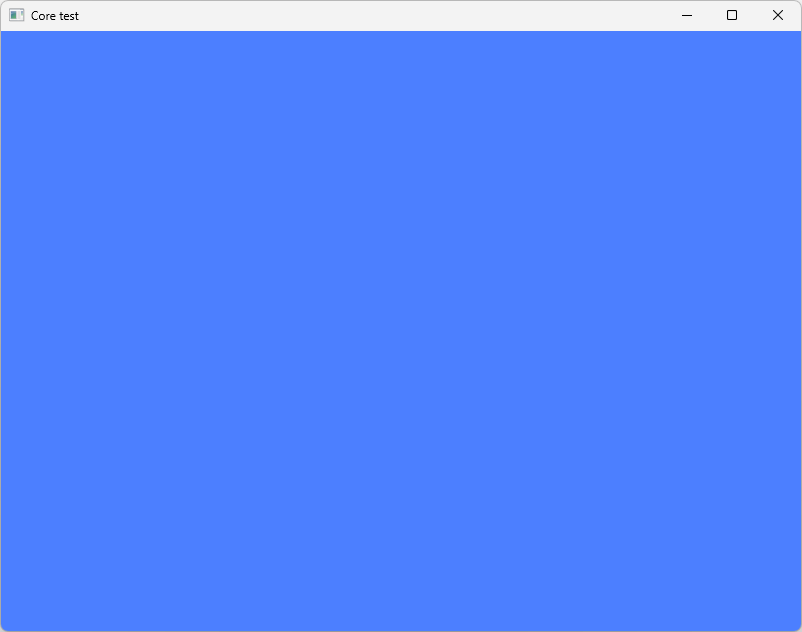
\includegraphics[width=\textwidth]{images/appendix_core_demo.png}
	\caption{Oczekiwany rezultat poprawnie skonfigurowanej aplikacji klienta dla modułu rdzeniowego.}
	\label{appendix_core_demo}
\end{figure}

\vfill
\clearpage

\subsection*{Warstwa silnika}
Na listingu \ref{lst:appendix:engineDemo} przedstawiony został kod aplikacji klienta, który testuje wszystkie krytyczne aspekty konfiguracji w przypadku użycia modułu silnika. Do poprawnego działania wymagany jest plik modelu sześcianu \textbf{cube.glb}, jako którego użyć można załączonego w repozytorium URM \cite{GitHub:Minik:MasterThesisUniversalRenderingModuleD3D11} pliku w lokalizacji \textbf{(...)/URMBenchmarks/Assets/cube.glb}. Plik ten musi znajdować się w folderze, z którego wywoływany będzie program. Można ten proces zautomatyzować dodając do niego referencję przy pomocy \textbf{Add -> Existing Item} po prawym kliknięciu na projekt aplikacji w Visual Studio, a następnie wybierając właściwości nowo dodanego pliku i zmieniając \textbf{General -> Item Type} na \textbf{Copy file}. Oczekiwany wynik został pokazany na rys. \ref{appendix_engine_demo}.

\begin{figure}[h!]
	\centering
	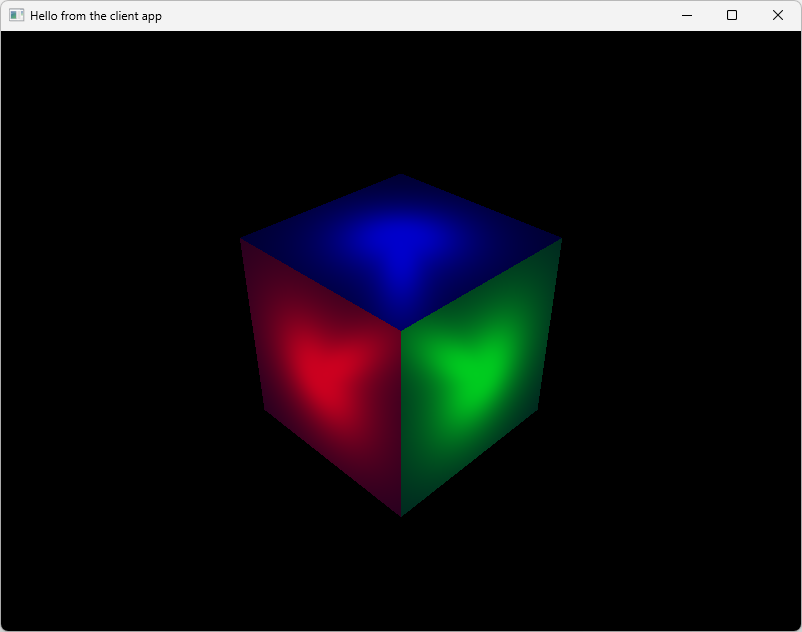
\includegraphics[width=\textwidth]{images/appendix_engine_demo.png}
	\caption{Oczekiwany rezultat poprawnie skonfigurowanej aplikacji klienta dla modułu silnika.}
	\label{appendix_engine_demo}
\end{figure}

\vfill
\clearpage

\begin{lstlisting}[caption={Aplikacja przykładowa wykorzystująca API modułu silnika}, label={lst:appendix:engineDemo}]
	#include <URM/Engine/Engine.h>
	#include <URM/Engine/CameraObject.h>
	#include <URM/Engine/ModelObject.h>
	
	int WinMain(HINSTANCE hInstance, HINSTANCE, LPSTR, int) {
		// Utworzenie modułu silnika
		URM::Engine::Engine engine(
			URM::Core::WindowCreationParams(800, 600, "Engine test", hInstance)
		);
		
		// Pobranie referencji do głównego obiektu sceny
		auto root = engine.GetScene().GetRoot();
		
		// Utworzenie kamery renderującej
		auto mainCamera = root.lock()->AddChild(new URM::Engine::CameraObject(45.0f));
		mainCamera->GetTransform().SetPosition({ 4.0f, 4.0f, 4.0f });
		mainCamera->GetTransform().LookAt({ 0.0f, 0.0f, 0.0f });
		engine.GetScene().SetMainCamera(mainCamera);
		
		// Utworzenie i dodanie do sceny czerwonego światła
		auto lightRed = root.lock()->AddChild(new URM::Engine::LightObject());
		lightRed->GetTransform().SetPosition({ 1.1f, 0.0f, 0.0f });
		lightRed->color = Color(1.0f, 0.0f, 0.0f, 1.0f);
		
		// Powtórzenie dla światła zielonego
		auto lightGreen = root.lock()->AddChild(new URM::Engine::LightObject());
		lightGreen->GetTransform().SetPosition({ 0.0f, 0.0f, 1.1f });
		lightGreen->color = Color(0.0f, 1.0f, 0.0f, 1.0f);
		
		// Oraz niebieskiego
		auto lightBlue = root.lock()->AddChild(new URM::Engine::LightObject());
		lightBlue->GetTransform().SetPosition({ -0.0f, 1.1f, 0.0f });
		lightBlue->color = Color(0.0f, 0.0f, 1.0f, 1.0f);
		
		// Wczytanie modelu sześcianu z pliku cube.glb
		auto object = root.lock()->AddChild(new URM::Engine::ModelObject("cube.glb"));
		
		// Uruchomienie pętli silnika
		engine.RunLoop();
		return 0;
	}
\end{lstlisting}